
Our task is to create a service, which classifies each text coming in a stream. The number of labels is considered to be multiple. The input elements come in two types. There are unlabelled texts, which topic is needed to obtain and labeled texts, which can be used in additional training. In the ~\ref{DSP}, we introduce systems that can be applied to our task, in ~\ref{DF} our computational pipeline explained in detail and in ~\ref{ML} ML model for additional fitting is shown.

\subsection{Distributed stream processing\label{DSP}}

In order to solve real-life tasks with high-velocity data, the stream processing systems can be used as a solution. The examples of such systems are Apache Flink [?], Google's MillWheel [?], Spark Streaming[?] or Apache Storm[?]. In these systems, every piece of data enters and exits the system one by one. Unlike batch-processing systems, this is done without any bufferization during the processing, which provides low latency for the elements. After entering, the elements are being transformed from one state to another by a map operation. 

For scalability, these systems are running on clusters of computers. To maximize the performance, calculations are evenly distributed among all computers. This method is called sharding technique. Usually, each element in streaming systems has a balancing function, which can be set by a user, for determining the shard, where further map transformations will be done with this element. That is, after each transformation every element can be sent to another machine using this scheme.

Stream processing systems have several issues to deal with. Most of them have a lack of determinism, which means that the result of computing is not the same between independent launches. Another issue is connected with the exactly-once delivery guarantee. This guarantee provides processing of each element by exactly one time. Other cases of processing it are at most one time and at least one time. The exactly-once guarantee is desirable, because valuable data should not be lost and, on the other hand, multiple processing of the same data causes latency.

In this work, our computations based on FlameStream \cite{kuralenok2018flamestream} distributed model, which provides the following advantages:

\textbf{Determinism.} This makes the whole classifying process more predictable as it was discussed in \cite{stonebraker20058} Rule 4. In addition, the concept ensures an opportunity for tests that validate the whole pipeline. FlameStream determinism is considered as lightweight.

\textbf{Exactly-once.} FlameStream process data in the exactly-once manner by default, which the same data processing on the Spark systems, for example, will be at a worse performance. The exactly-once guarantee ensures a low latency with almost no overhead.

These advantages allow us to create a classifier with predictable results and due to the exactly-once delivery guarantee provide low latency.

\subsection{Data flow \label{DF}}

\subsubsection{Computational pipeline}

Similar to other stream processing systems, FlameStream sets scheme of calculations by a computational graph. This graph is commonly referred to as a logical graph. For our task, the calculations can be illustrated as a logical graph below:

\begin{figure}[htbp]
  \centering
  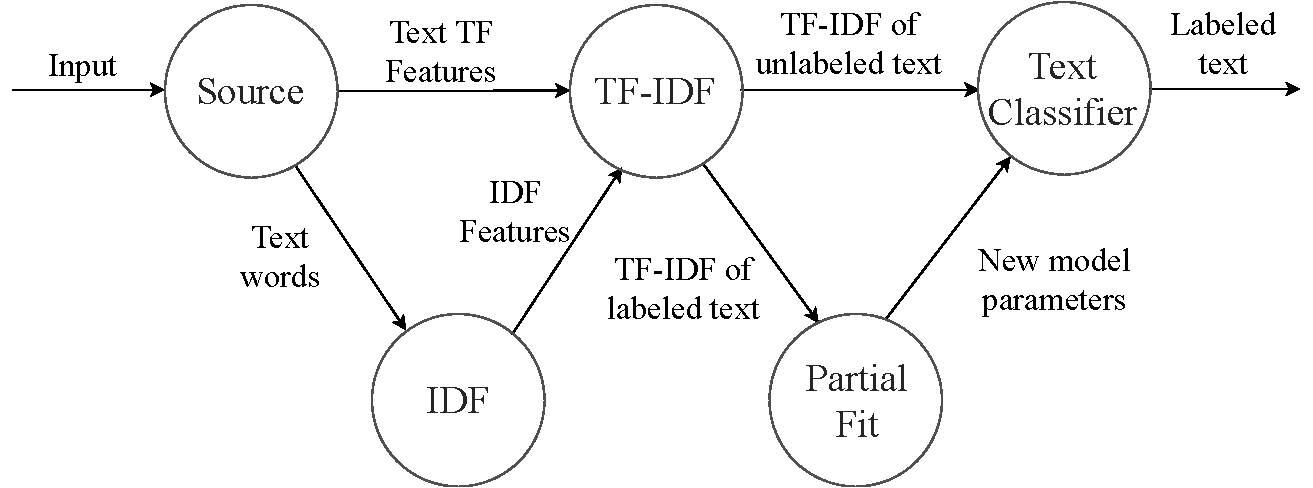
\includegraphics[scale=0.48]{pics/logical-graph}
  \caption{The logical pipeline}
  \label {logical graph}
\end{figure}

An oriented edge indicates the flow and kind of data. Every vertex in the graph represents a transform operation with the data. Text Document vertex receives incoming texts, calculates term frequencies and transfers it to the TF-IDF vertex. Also, for each text, this vertex obtains a word list in the text and sends it to IDF vertex. The results of the IDF vertex are delivered to the TF-IDF vertex, where TF-IDF features of the text are joined together with TF features, which were calculated in the previous step. After that, the unlabelled text is sent to Text Classifier vertex, where its topic is obtained and the result is delivered to the user.

\begin{figure}[htbp]
  \centering
  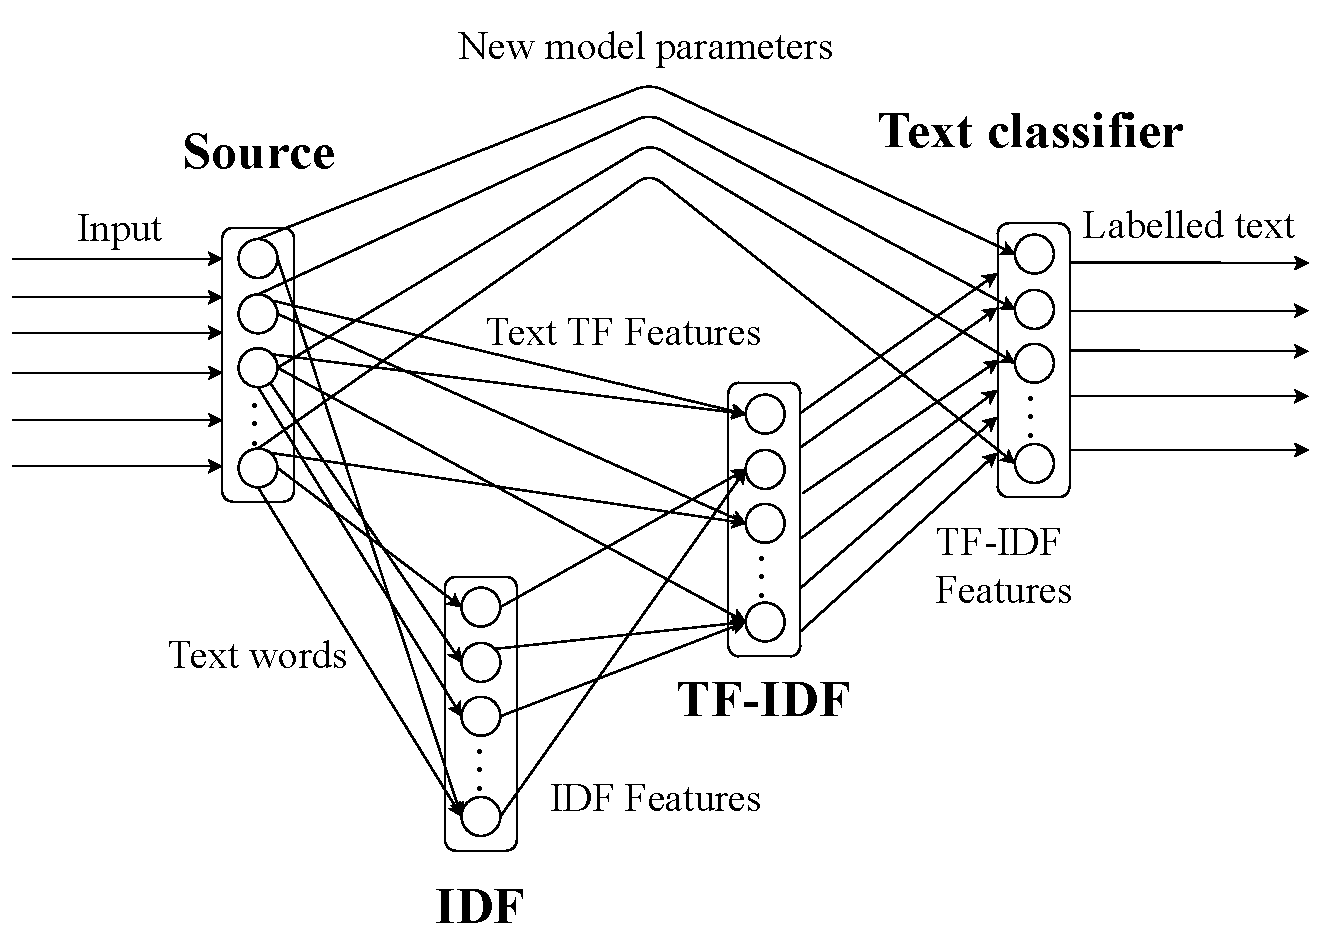
\includegraphics[scale=0.375]{pics/physical-graph}
  \caption{The physical pipeline}
  \label {physical graph}
\end{figure}

These computations map into a physical graph of the pipeline, which showed in Figure ~\ref{physical graph}. This graph defines the real flow of data. Every vertex here is a single machine. Each rectangle denotes the same cluster of computers.

For evenly spread workload the Stream processing systems apply a balancing function for each element. The function is set by a user. In FlameStream case, we use a hash function for the distributing. The range $[0, 2^{32}-1]$ is divided into equal parts by the number of the shards. Every single shard is responsible for its own range. Hash of each element defines what shard will be used for further computation.

That is, real calculations are defined by the physical graph and can be described as follows. Input text can be received by any machine. Then Text Document vertex produces a list of words for the text and the list is distributed among all shards using the described scheme. In case of words with a high frequency such as conjunctions or prepositions, we add to them salt to the end thereby spreading all the words between the shards evenly. After that, a list of words distributed among all shards for IDF processing using the technique. In the TF-IDF stage, IDF features of the same document accumulate on a particular shard using the scheme. In the IDF and TF-IDF stages the same sharding method is used, however, the difference is during IDF processing sharding is done by a word and during TF-IDF -- by a text document. Accumulated IDF features join with the corresponding TF features. In the Text Classifier stage, classifier obtains a label for the text and returns it to the user. During this stage, the classifying process is done on the same machine, where TF-IDF features were gathered together.

\subsubsection{Dealing with concept drift}

Concept drift is a phenomenon of changing users' interests from time to time, which usually depends on recent events, and results in shifting the distribution of text classes to particular ones. Essentially, this may affect the correctness of the pipeline, more specifically, the computing of the IDF features. To overcome the issue, we use windowed IDF calculation: concrete IDF values will be provided based on input within a time window. For instance, the window can be set to a day or a week. This scheme allows us to deal with sudden changes in the topics.

\subsubsection{Partial fit}

Figures ~\ref{logical graph}, ~\ref{physical graph} provide a scheme for a partial fitting. Some of the text documents labeled and such documents accumulate in the Partial Fit vertex. Additional training is triggered by a special element, which is submitted to the input as text documents. However, this element is not processed as text and the vertices push the element further. This process is similar to punctuation processing \cite{tucker2003exploiting}. The conditions, when the partial fitting starts, can be chosen arbitrarily by a system administrator, for example, train on every 10000 documents. During this process, the existing classifier's parameters can be updated.

\subsection{ML model \label{ML}}

The classifier's model can be chosen independently from other computations. In our case, we use Multinomial Logistic Regression. At the start of the system, the initial classifier parameters such as weights can be provided by a pre-train process, which is, in our case, executed using the sklearn library. We vectorize texts using TfidfTransformer class and the model fits the documents by SGDClassifier class with l1 regularization. The regularization provides us weights as a sparse matrix.

Every time, when the Partial Fit is triggered, the following process occurs, which can be described in terms of the optimization of a cost function. This function in our case is written below:

\begin{center}

$$ J(W) = -\frac{1}{m} \sum \limits_{i = 1}^{m} \sum \limits_{j = 1}^{k} \mathbbm{1}_{\left\{y^{(i)} == j\right\}} \cdot \log \frac{\exp\left({W_{j}^Tx^{(i)}}\right) }{\sum \limits_{l = 1}^{k}  \exp\left({W_{l}^Tx^{(i)}}\right) }$$ 
 $$ +  \lambda_1 ||W||_1 + \lambda_2 ||W - W_{prev}||_2 $$

\end{center} 

The number of points in a new dataset is denoted as $m$. The point with index $i$ showed as $x^{(i)}$. The number of classes is $k$. New weights are designated as $W$. The weights, that computed in the previous step, are $W_{prev}$. At the first time of triggering the process, $W_{prev}$ are the weights, that received fromfrom sklearn script. 

The formula provides the goal of the training. The first component is the standard softmax function for multiple classes. The second component keeps the l1 regularization of the weights. To use the previous history of the classifier weights we apply l2 regularization as the third component. Fitting new points and the consideration of the previous weights ensure better accuracy of the classifier.

We are interested in finding such $W$ that minimizes $J(W)$. Taking derivatives, one can show that the gradient for each class component is:

\begin{center}

$$ \nabla_{W_j} \; J(W) = -\frac{1}{m} \sum \limits_{i = 1}^{m} \left[ x^{(i)} \left( \mathbbm{1}_{\left\{y^{(i)} == j\right\} } - \frac{\exp\left({W_{j}^Tx^{(i)}}\right)}{\sum \limits_{l = 1}^{k}  \exp\left({W_{l}^Tx^{(i)}}\right)} \right) \right] $$
$$ - \; \lambda_1 sign\left(W\right) - \frac{\lambda_2}{2} \left(W - W_{prev} \right), \; j = [1..k] $$

\end{center} 

This formula is applied to each component during one step of gradient descent. There are a few steps of the gradient is executed and new models' parameters are distributed among shards for further classification.